\documentclass[10pt]{article}
\usepackage{wrapfig}
%\usepackage{epsf}
\usepackage{fancyhdr,epsfig,graphics,tabularx,times}
\usepackage{amsmath}
\usepackage{amssymb}
\usepackage{palatino}
%\usepackage[dvips]{graphics}
\usepackage{fancyhdr}
\usepackage{epsfig}
\usepackage{multirow}
\usepackage{cancel}
\usepackage[bookmarks]{hyperref}
\usepackage{longtable}
\usepackage{soul}
\parindent 0in
\parskip 1ex
\oddsidemargin  0in
\evensidemargin 0in
\textheight 8.5in
\textwidth 6.5in
\topmargin -0.25in
\setcounter{section}{0}

\pagestyle{fancy}
\lhead{\bf BME354L: Introduction to Medical Instrumentation}
\rhead{\bf Nightingale (Spring 2015)}
\cfoot{\thepage}



\begin{document}

\section*{Variables and Functions in Arduino}

Programming in Arduino's C language is very different than the majority of programming that you have done so far in the engineering curriculum, which heavily utilizes Matlab. This may create a steep learning curve, but once you gain a hold of the syntax, programming the Arduino will not be that difficult. One of the biggest differences between C and Matlab is how functions and variables are declared and used. 
This document will highlight the differences in program structure, functions, and variables to help get you started.

\subsection*{Basic Arduino Set-Up}
A \textit{sketch} is the name Arduino uses for programs.  It is the unit of code that is uploaded to and run on an Arduino board.  All sketches \textbf{must} have 2 void type functions, \texttt{setup()} and \texttt{loop()}. "Void" simply means that the function doesn't return any value. 
\par The \texttt{setup()} method is run once just after the Arduino is powered on, and the \texttt{loop()} is run continuously afterwards.  The \texttt{setup()} is where you want to do any initialization steps, and in \texttt{loop()}, you want to run the code you want to run over and over again.  Your basic sketch should look something like this:

\begin{figure}[h]
\centering
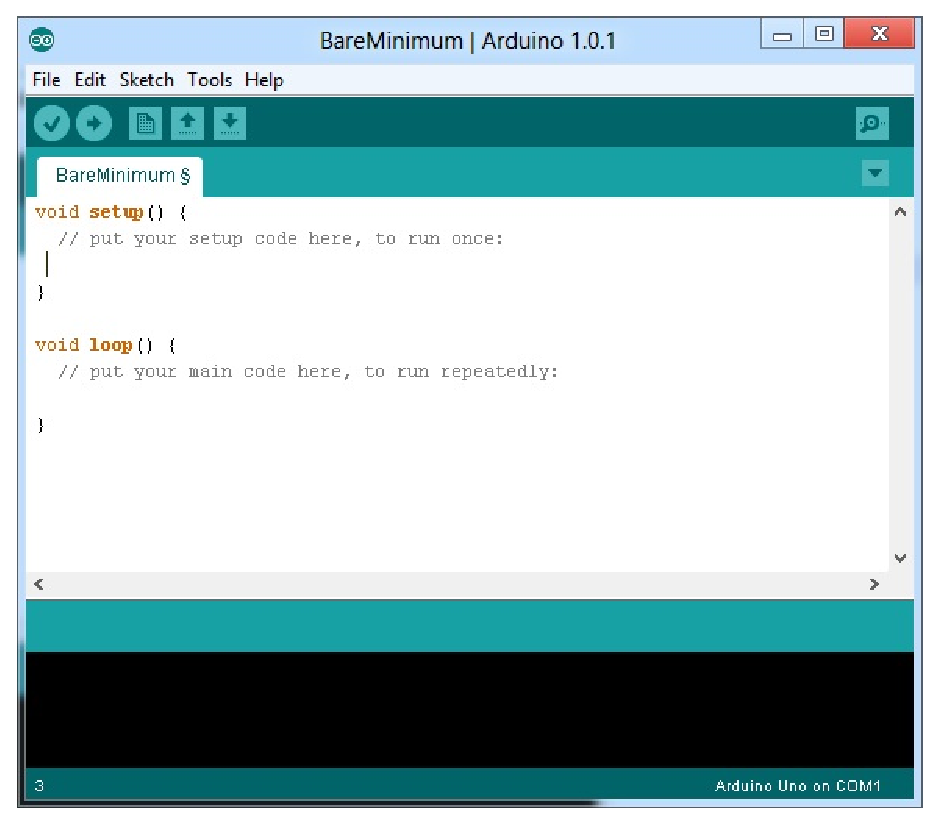
\includegraphics[width=4in]{pics/arduino_bareminimum.eps}
\caption{Bare minimum code required for an Arduino sketch}
\label{fig:arduino_bareminimum}
\end {figure}

\subsection*{Variables}
A variable is a place to store a piece of date. It has a name, a type, and a value.
\par \textbf{Name:} You can name a variable any word that is not already a keywords in Arduino. You should also avoid beginning variable names with numeral characters

\par \textbf{Type:} Unlike Matlab, you must declare all variable types before using them when coding in Arduino. In choosing a variable type, it is important to consider the size of the numbers you want to store. Variables will roll on when the value stored exceeds the space assigned to store it. Here are some common variable types:

\begin{center}
\begin{tabular}{l p{7.5cm} l l}
\textbf{Name} & \textbf{Description} & \textbf{Range of Values} & \textbf{Size} \\ \hline
\texttt{int} & Integer, primary data-type for number storage & -32,768 \mbox{--} 32,767 & 2 bytes \\ \hline
\texttt{long} & Extended size variable for number storage & -2,147,483,648 \mbox{--} 2,147,483,647 & 4 bytes \\ \hline
\texttt{float} & Floating point numbers, used for numbers that have a decimal point. Floating numbers allow for 6-7 points of data precision.  However, math with float variable is significantly slower. & -3.402835\mbox{\textsc{e}}38 \mbox{--} 3.402835\mbox{\textsc{e}}38 & 4 bytes \\ \hline
\texttt{double} & Double precision floating number. These take up 4-bytes on the Arduino UNO - the same as float variables - so even with double implementation, there is no gain in precision. & -3.402835\mbox{\textsc{e}}38 \mbox{--} 3.402835\mbox{\textsc{e}}38 & 4 bytes \\ \hline
\texttt{byte} & Stores an 8-bit unsigned number & 0 \mbox{--} 255 & 1 byte \\ \hline
\texttt{boolean} & Holds one of two values, true or false & true/false & 1 byte \\ \hline
\end{tabular}
\end{center}

Variables can also be \texttt{unsigned}.  This is helpful when dealing solely with positive numbers, as it can essentially double the range of useful values.  For example \texttt{unsigned int} can hold values from 0 to 65,535. 

When declaring variables, the location of variable declaration matters, and variables can be \textit{global} or \textit{local}.

A global variable is declared outside of a function (e.g. \texttt{setup()}, \texttt{loop()}, etc.), and can be seen by every function in the program.  

A local variable is declared within a function and can only be seen by that function. Local variables are useful when programs start to become larger and complex.  They insure that only one function has access to its own variables and prevents programming errors when one function may accidentally modify same-name variables used by another function. 

\par \textbf{Value:} When declaring a variable, setting an initial value is \textit{optional}. For example:
\par \hspace{4ex} \texttt{unsigned int Variable1;}
\par \hspace{4ex}  \texttt{unsigned int Variable2=0;}
\par Both are correct ways to declare variables. It is often to useful to initialize variables, but it will be dependent on the information that the variable is actually storing. 

\subsection*{Functions}

\subsubsection*{Creating Modular Code}
When coding in Arduino, it is best to use functions and make your code as modular as possible, for a number of reasons:

\begin{itemize}
\item Helps the keep the program organize and often helps to conceptualize the program
\item Makes the code more readable and easier to debug by codifying the one action in one place
\item Makes the whole sketch smaller when sections of code are reused many times
\item Makes it easier to reuse code in other programs
\end{itemize}

As you know, Arduino sketches require 2 functions: \texttt{setup()} and \texttt{loop()}.  All other functions must be created outside the brackets of those two functions. In making your own function, it is helpful to designate a \textbf{New Tab} in your Arduino sketch to the function. The Arduino website provides a helpful diagram of the basic structure of functions:

\begin{figure}[ht]
	\centering
	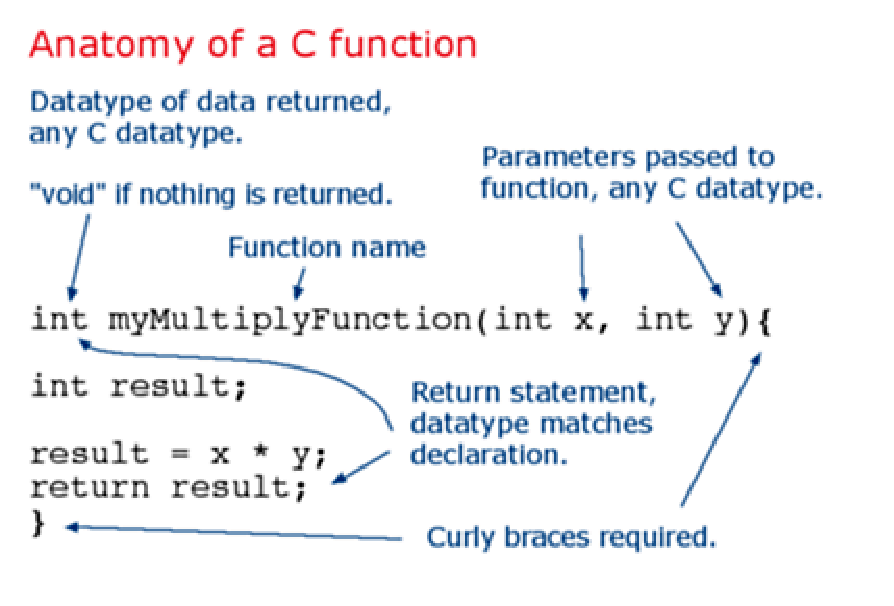
\includegraphics[height=2in]{pics/c_function_anatomy.eps}
	\caption{Anatomy of a C Function.}
	\label{c_function_anatomy}
\end{figure}

To "call" on this simple multiplication function, we pass it the parameters of interest.
\par \hspace{4ex} \texttt{ans = myMultiplyFunction(4,6); // ans now contains the value 24}

\end{document}
